\documentclass{standalone} 

\usepackage{tikz}
\usetikzlibrary{arrows.meta,shapes, calc, fit, patterns, positioning, intersections, 3d, matrix, angles, quotes, backgrounds}

\begin{document}

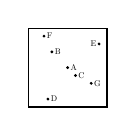
\begin{tikzpicture}

    \draw[] (0,0) rectangle (1cm,1cm);

    \draw[fill] (0.5cm,0.5cm) circle (0.01cm) node[anchor=west,transform shape,scale=0.3]{A};
    \draw[fill] (0.3cm,0.7cm) circle (0.01cm) node[anchor=west,transform shape,scale=0.3]{B};
    \draw[fill] (0.6cm,0.4cm) circle (0.01cm) node[anchor=west,transform shape,scale=0.3]{C};
    \draw[fill] (0.25cm,0.1cm) circle (0.01cm) node[anchor=west,transform shape,scale=0.3]{D};
    \draw[fill] (0.9cm,0.8cm) circle (0.01cm) node[anchor=east,transform shape,scale=0.3]{E};
    \draw[fill] (0.2cm,0.9cm) circle (0.01cm) node[anchor=west,transform shape,scale=0.3]{F};
    \draw[fill] (0.8cm,0.3cm) circle (0.01cm) node[anchor=west,transform shape,scale=0.3]{G};

\end{tikzpicture}

\end{document}
